% !TEX program = xelatex
% 数学物理方法1 · 第四章专题 · 大圆弧引理与小圆弧引理
\documentclass[11pt]{ctexart}
%=====================================================================
% theme-violet.tex —— 讲义精讲 · 紫花主题
% 用法：\documentclass[11pt]{ctexart}
%       \input{assets/theme-violet}
%       \begin{document} ... \end{document}
% 只用 ctexart 自带能力 + xcolor/enumitem/fancyhdr/pifont/amsmath，
% 不依赖 tikz/tcolorbox，保证 MiKTeX 可直接编译。
%=====================================================================

\usepackage[a4paper,left=2.0cm,right=2.0cm,top=2.1cm,bottom=2.3cm,%
            headsep=12pt,footskip=22pt]{geometry}
\usepackage{amsmath,amssymb}
\usepackage{needspace}
\usepackage{xcolor}
\usepackage{array}
\usepackage{enumitem}
\usepackage{pifont}
\usepackage{fancyhdr}
\usepackage[hidelinks]{hyperref}

%---------------------------------------------------------------- 配色
\definecolor{violet}{RGB}{107,78,143}      % 主色：紫
\definecolor{violetdeep}{RGB}{63,44,92}    % 深紫：标题/强调
\definecolor{petal}{RGB}{183,159,208}      % 花瓣：装饰线、花饰
\definecolor{bandviolet}{RGB}{247,243,251} % 浅紫底：档案/提示框
\definecolor{bandcream}{RGB}{252,249,242}  % 米白底：易错/注意框
\definecolor{rulepurple}{RGB}{217,207,230} % 分隔线
\definecolor{inkgray}{RGB}{92,96,110}      % 次要文字

%---------------------------------------------------------------- 字体
% 有 Noto CJK 用 Noto，没有就退回 ctex 默认（Windows 下为宋体/黑体）
\IfFontExistsTF{Noto Serif CJK SC}{\setCJKmainfont{Noto Serif CJK SC}}{}
\IfFontExistsTF{Noto Sans CJK SC}{\setCJKsansfont{Noto Sans CJK SC}}{}

%---------------------------------------------------------------- 版式
\setlist{nosep,leftmargin=1.9em}
\linespread{1.28}
\setlength{\parskip}{3.5pt}
\setlength{\parindent}{0pt}
\setlength{\tabcolsep}{5pt}
\renewcommand{\arraystretch}{1.28}

%---------------------------------------------------------------- 花饰
% \ding{95} = 五瓣小花，\ding{96} = 星形花；都来自 pifont，必定存在
\newcommand{\orn}{\textcolor{petal}{\ding{95}}}          % 行内小标
\newcommand{\ornstar}{\textcolor{petal}{\ding{96}}}      % 星形花
\newcommand{\flowerrule}{%                                % 居中花饰分隔线
  \par\vspace{7pt}%
  \noindent\makebox[\linewidth]{\color{petal}%
    \rule{0.20\linewidth}{0.6pt}\hspace{8pt}{\small\ding{95}}\hspace{4pt}%
    \raisebox{1.1pt}{\tiny\ding{95}}\hspace{4pt}{\small\ding{95}}\hspace{8pt}%
    \rule{0.20\linewidth}{0.6pt}}%
  \par\vspace{7pt}}

%---------------------------------------------------------------- 标题与节头
\newcommand{\doctitle}[3]{%   #1 主标题  #2 副标题  #3 元信息（可用 \\ 分行）
  \begin{center}
    {\color{petal}\small \orn\enspace #2\enspace \ornstar}\\[7pt]
    {\LARGE\bfseries\color{violetdeep} #1}\\[10pt]
    {\color{petal}\rule{0.55\linewidth}{1pt}}\\[4pt]
    {\small\color{inkgray} #3}
  \end{center}\vspace{2pt}}

\newcommand{\hdr}[2]{%   #1 章节号（如 §0）  #2 标题
  \par\vspace{12pt}%
  \noindent\colorbox{violetdeep}{\color{white}\bfseries\small\;#1\;}\hspace{7pt}%
  {\color{violetdeep}\large\bfseries #2}\par\nobreak
  \vspace{3pt}{\color{petal}\hrule height 1.2pt}\vspace{6pt}}

\newcommand{\subhdr}[1]{%
  \par\vspace{6pt}%
  \noindent{\color{violet}\bfseries #1}\par\vspace{1pt}}

%---------------------------------------------------------------- 提示框
\newcommand{\callout}[1]{% 浅紫底：讲义档案、读法说明
  \par\medskip\noindent
  \fcolorbox{rulepurple}{bandviolet}{\parbox{\dimexpr\linewidth-2\fboxsep-2\fboxrule}{\vspace{2pt}#1\vspace{2pt}}}%
  \par\medskip}

\newcommand{\warnbox}[1]{% 米白底：易错、边界条件
  \par\medskip\noindent
  \fcolorbox{rulepurple}{bandcream}{\parbox{\dimexpr\linewidth-2\fboxsep-2\fboxrule}{\vspace{2pt}#1\vspace{2pt}}}%
  \par\medskip}

\newcommand{\gapitem}[2]{% #1 缺口类型（紫） #2 内容
  \par\vspace{2pt}\noindent
  \hangindent=1.4em\hangafter=1
  {\color{petal}\small\ding{96}}\enspace{\bfseries\color{violetdeep}#1}\enspace #2\par}

% 题干块（\qstem）：每道例题／作业的「详解」开头必须先复述题干与出处。
% 起因：2026-10-25 第五章讲义把七道作业的题面集中放在一页、详解另起一页，
% 读者翻到「第 4 题」时看不到条件，等于一道没有题干的题目。
% 规则：详解块内自带题干，读者不翻页就能读懂题在问什么。
\newcommand{\qstem}[1]{%
  \par\medskip\noindent
  \fcolorbox{violet}{bandviolet}{%
    \parbox{\dimexpr\linewidth-2\fboxsep-2\fboxrule}{%
      \vspace{2pt}%
      {\small\bfseries\color{violet}题干}\hspace{0.8em}#1%
      \vspace{2pt}}}%
  \par\medskip}

% v2: 保护题干与开头，长题可跨页，续页补上下文。
\newcommand{\qbreak}{\needspace{6\baselineskip}}
% 独立练习：ID、来源、题干、考点、答案标签（通常 ans:ID）。
\newcommand{\practice}[5]{%
  \qbreak\subhdr{练习 #1}\qstem{（#2）#3}%
  \textbf{考点}：#4\par
  详解见附录第~\pageref{#5}~页。\par\medskip}
% 附录开头：ID、来源、条件摘要；自动产生 ans:ID 标签。
\newcommand{\answerstart}[3]{%
  \qbreak\subhdr{#1\quad 详解}\label{ans:#1}\qstem{（#2）#3}}
\newcommand{\answercontinue}[2]{%
  \needspace{5\baselineskip}\subhdr{#1\quad 续解}%
  {\small\color{inkgray}本页接续：#2}\par\medskip}
% 延迟提供默认值，让旧讲义可在导言区保留自己的 \newcommand{\step}。
\AtBeginDocument{\providecommand{\step}[1]{\needspace{3\baselineskip}\par\medskip\textbf{#1}\par}}

% 前提旁注：只放在「需要理解的那一步」后面，给陈述 + 本题代入，不重证。
\newcommand{\aside}[1]{%
  \par\vspace{1pt}\noindent
  \hangindent=1.6em\hangafter=1
  {\small\color{inkgray}%
    \hspace*{0.6em}{\color{petal}$\triangleright$}\hspace{2pt}#1}%
  \par\vspace{2pt}}

%---------------------------------------------------------------- 表格
% 本机 MiKTeX 的 colortbl 与 array 版本不匹配（\rowcolor 会报错），
% 故表格统一用「上粗紫线 + 表头 + 中细线」的三线式，不依赖 colortbl。
\newcommand{\tabtop}{\par\vspace{3pt}{\color{violet}\hrule height 1.2pt}\vspace{1pt}}
\newcommand{\tabmid}{\par\vspace{1pt}{\color{petal}\hrule height 0.5pt}\vspace{1pt}}
\newcommand{\tabbot}{\par\vspace{3pt}{\color{rulepurple}\hrule height 0.5pt}\vspace{8pt}}
\newcommand{\thead}[1]{{\bfseries\color{violetdeep}#1}}

%---------------------------------------------------------------- 页眉页脚
\pagestyle{fancy}
\fancyhf{}
\renewcommand{\headrulewidth}{0.4pt}
\renewcommand{\headrule}{\hbox to\headwidth{\color{rulepurple}\leaders\hrule height \headrulewidth\hfill}}
\fancyhead[L]{\small\color{inkgray}\songti \doctag}
\fancyhead[R]{\small\color{inkgray}\songti \coursetag}
\fancyfoot[C]{\small\color{inkgray}\orn\enspace{\color{violet}\thepage}\enspace\orn}

% 每篇讲义在导言区设这两个值
\newcommand{\doctag}{}
\newcommand{\coursetag}{}
\newcommand{\settags}[2]{\renewcommand{\doctag}{#1}\renewcommand{\coursetag}{#2}}

%---------------------------------------------------------------- 数学记号
\newcommand{\vect}[1]{\boldsymbol{#1}}
\newcommand{\dd}{\,\mathrm{d}}
\newcommand{\ddx}{\frac{\mathrm{d}}{\mathrm{d}x}}
\addtolength{\jot}{2pt}



\usepackage{tikz}
\usetikzlibrary{arrows.meta}
\settags{第四章专题 · 大圆弧引理与小圆弧引理}{数学物理方法1}

\renewcommand{\qbreak}{\needspace{0.45\textheight}}
\let\origsubhdr\subhdr
\renewcommand{\subhdr}[1]{\par\needspace{4\baselineskip}\origsubhdr{#1}}
\let\orighdr\hdr
\renewcommand{\hdr}[2]{\par\orighdr{#1}{#2}}
\setlength{\abovedisplayskip}{7pt plus 2pt minus 2pt}
\setlength{\belowdisplayskip}{7pt plus 2pt minus 2pt}

\begin{document}

\doctitle{第四章专题　大圆弧引理与小圆弧引理}
{围道两端的两个极限：$R\to\infty$ 与 $\varepsilon\to0$}
{配合课件《第四章 留数定理及应用》§4.3\quad 2026-11-02\quad 数学物理方法1}

\hdr{§0}{这份讲义要解决什么}

留数定理把围道积分换成留数之和，但它有一个前提：围道必须是\textbf{闭合}的。实轴上的积分是开区间，要先用两段弧把它补成闭合围道——上半平面的大圆弧 $C_R$，以及绕过实轴上极点的小圆弧 $C_\varepsilon$。补上以后，多出来的这两段积分必须能“扔掉”，否则等式不成立。

扔掉它们靠的就是本专题的两个引理：

- \textbf{大圆弧引理}：$R\to\infty$ 时，若 $|f|$ 掉得足够快，大圆弧上的积分趋于 0。
- \textbf{小圆弧引理}：$\varepsilon\to0$ 时，若极点是一阶的，小圆弧上的积分趋于 $-i\pi$ 乘留数（于是留下一个“半留数”）。

两个引理都只是 ML 不等式的一次应用，但用法和条件完全不同，混用会直接算错。下面把两个引理分开讲透，再讲它们怎么配合。

\subhdr{0.1\quad 第一次出现的新概念（后面每个都会展开）}

\begin{itemize}
\item \textbf{围道的“补弧”}：把开区间 $(-\infty,\infty)$ 补成一个闭合曲线的做法（§2.1、§3.1）。
\item \textbf{一致上界 $M(R)$}：在整条弧上都能用的界，不是某一点的最大值（§1.1）。
\item \textbf{柯西主值}（$\mathrm{PV}$）：实轴上有极点、普通积分发散时，用对称挖洞定义的“广义值”（§3.7）。
\item \textbf{半留数}：小圆弧只绕过一圈的一半，于是贡献是 $i\pi\operatorname{Res}$ 而不是 $2\pi i\operatorname{Res}$（§3.8）。
\item \textbf{约当引理}：当 $|f|$ 只按 $1/R$ 衰减、大圆弧引理失效时，用 $e^{imz}$ 的振荡把积分压到 0 的工具（§2.6）。
\end{itemize}

\subhdr{0.2\quad 记号}

\begin{itemize}
\item $C_R$：上半平面大圆弧 $z=Re^{i\theta}$，$\theta\in[0,\pi]$（从 $R$ 走到 $-R$）。
\item $C_\varepsilon$：以实轴上的点 $a$ 为心、半径 $\varepsilon$ 的小半圆。
\item $L$：弧长；$M$：被积函数在弧上的上界。
\item $\mathrm{PV}\!\int$：柯西主值；$\operatorname{Res}$：留数（第四章 §1）。
\end{itemize}

\hdr{§1}{唯一的工具：ML 不等式}

\subhdr{1.1\quad 陈述与证明}

\textbf{引理（ML 不等式）}：设 $f$ 在曲线 $C$ 上连续，$L$ 是 $C$ 的长度，且

$$
|f(z)|\le M\qquad(z\in C).
$$

则

$$
\left|\int_C f(z)\,\mathrm{d}z\right|\le ML .
$$

\textbf{证明}：把积分写成黎曼和的极限，用“和的模不超过模的和”，再取极限：

$$
\left|\int_C f\,\mathrm{d}z\right|
=\lim\left|\sum_k f(z_k)\Delta z_k\right|
\le\lim\sum_k |f(z_k)|\,|\Delta z_k|
\le M\lim\sum_k|\Delta z_k|
= M L .
$$

这里最后一个等号是弧长的定义（分割细到极限）。

\textbf{另一种写法（参数化，考试里更常用）}：设 $C$ 的参数方程是 $z=z(t)$，$t$ 从 $\alpha$ 到 $\beta$，则

$$
\left|\int_C f\,\mathrm{d}z\right|
=\left|\int_\alpha^\beta f(z(t))z'(t)\,\mathrm{d}t\right|
\le\int_\alpha^\beta |f(z(t))|\,|z'(t)|\,\mathrm{d}t
\le M\int_\alpha^\beta|z'(t)|\,\mathrm{d}t=ML ,
$$

因为 $\int_\alpha^\beta|z'(t)|\mathrm{d}t$ 正是弧长。

\subhdr{1.2\quad 使用要点（两个都容易踩错）}

\textbf{第一，$M$ 必须是整条弧上的上界，不能取某一点的值}。例如 $f=e^{iz}/z$ 在 $C_R$ 上，$z=Re^{i\pi/2}=iR$ 处模很小（$e^{-R}/R$），但靠近实轴的两端 $\theta\approx0,\pi$ 处模约为 $1/R$。用 $M=1/R$ 才是对的，用最小值会得出错误结论。

\textbf{第二，$L$ 是弧长，不是半径}。上半圆弧长是 $\pi R$，不是 $R$，也不是 $2\pi R$（那是整圆）。这两个常数经常被写混，差一个 $2$ 或 $\pi$ 就让“趋于零”变成“不趋于零”。

\subhdr{1.3\quad 一个“恰好取等”的例子}

取 $f(z)=1/z$，$C$ 是上半大圆弧 $C_R$。弧长 $\pi R$，而 $|f|=1/R$，所以 $ML=\pi$。实际计算：

$$
\int_{C_R}\frac{\mathrm{d}z}{z}
=\int_0^{\pi}\frac{iRe^{i\theta}}{Re^{i\theta}}\,\mathrm{d}\theta
=i\pi .
$$

积分值就是 $i\pi$，模为 $\pi$ —— ML 不等式的界被\textbf{取到}了。这个例子说明：对大圆弧上的 $1/z$，任何估计都不可能给出 0，因为它真的不趋于 0。

\hdr{§2}{大圆弧引理}

\subhdr{2.1\quad 情境：为什么需要补一条弧}

要算实轴上的积分

$$
\int_{-\infty}^{\infty}f(x)\,\mathrm{d}x ,
$$

可以补一条上半大圆弧 $C_R$，把 $[-R,R]$ 与 $C_R$ 拼成闭合围道 $\Gamma_R$。围道闭合了，留数定理就能用：

$$
\int_{-R}^{R}f(x)\,\mathrm{d}x+\int_{C_R}f(z)\,\mathrm{d}z
=2\pi i\!\!\sum_{\text{上半平面}}\!\operatorname{Res}f .
$$

要让左边第一项在 $R\to\infty$ 时就是要求的实积分，必须让第二项趋于 0。这就是大圆弧引理要保证的事。

\begin{center}
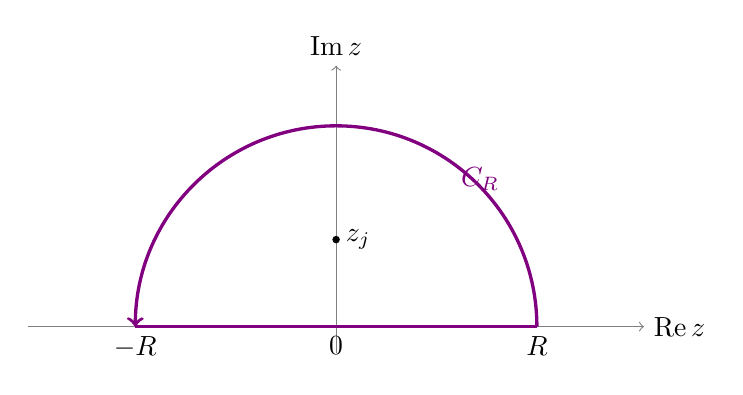
\begin{tikzpicture}[scale=0.85]
\draw[->,gray] (-4.6,0) -- (4.6,0) node[right,black]{$\mathrm{Re}\,z$};
\draw[->,gray] (0,-0.4) -- (0,3.9) node[above,black]{$\mathrm{Im}\,z$};
\draw[violet,very thick] (-3,0) -- (3,0);
\draw[violet,very thick,->] (3,0) arc (0:180:3);
\node[violet] at (2.15,2.2) {$C_R$};
\fill (0,1.3) circle (1.6pt) node[right,black]{$z_j$};
\node[below] at (0,0) {$0$};
\node[below] at (3,0) {$R$};
\node[below] at (-3,0) {$-R$};
\end{tikzpicture}
\end{center}

图上这条闭合曲线 $\Gamma_R$ 由实轴段与上半大圆弧拼成；$z_j$ 是上半平面里的奇点。留数定理对它成立，前提是实轴段上\textbf{没有}奇点（有的话就要挖洞，见 §3）。

\subhdr{2.2\quad 陈述}

\textbf{引理（大圆弧引理）}：设 $f$ 在 $C_R$ 上连续，且

$$
|f(z)|\le M(R)\qquad(z\in C_R),
$$

若

$$
R\,M(R)\to0\qquad(R\to\infty),
$$

则

$$
\int_{C_R}f(z)\,\mathrm{d}z\to0 .
$$

\textbf{证明}：由 ML 不等式，弧长 $L=\pi R$，

$$
\left|\int_{C_R}f\,\mathrm{d}z\right|
\le M(R)\cdot \pi R
=\pi\bigl(R\,M(R)\bigr)\to0 .
$$

\aside{条件里的 $\pi$ 不影响结论：只要是常数倍的 $R\,M(R)$，趋于 0 就是趋于 0。所以判定时只看“$|f|$ 是否比 $1/R$ 掉得快”，不必纠结常数。}

\subhdr{2.3\quad 三种等价写法}

\textbf{写法一（本讲义主用）}：$R\,M(R)\to0$。

\textbf{写法二（幂次形式）}：若 $|f(z)|\le C/R^{1+\delta}$（$\delta>0$），则 $\pi R\,CM/R^{1+\delta}=\pi C/R^{\delta}\to0$。教材常写成“$|f|$ 在无穷远像 $1/z^{1+\delta}$”。

\textbf{写法三（圆心不在原点）}：若 $C_R$ 是以 $z_0$ 为心的圆弧，弧上 $|z|\le R+|z_0|=O(R)$，所以只要 $R\,M(R)\to0$，结论不变。但此时弧长仍是 $\pi R$，不是 $\pi(R+|z_0|)$。

\subhdr{2.4\quad 典型用法：有理函数为什么要求“次数差两次”}

设

$$
f(z)=\frac{P(z)}{Q(z)},\qquad \deg Q\ge \deg P+2 .
$$

$|z|=R$ 很大时，分子像 $R^{m}$、分母像 $R^{n}$，所以

$$
|f|\sim \frac{C}{R^{\,n-m}},\qquad n-m\ge2 .
$$

于是

$$
R\,M(R)\sim \frac{C}{R^{\,n-m-1}}\le\frac{C}{R}\to0 .
$$

\textbf{只差一次时}（$n=m+1$），$R\,M\sim C$ 是常数，大圆弧引理给不出零。这时候积分本身可能仍然收敛（例如 $\int x/(1+x^2)$ 是奇函数的主值），但大圆弧上的积分不会消失——补弧的办法失败。

\subhdr{2.5\quad 两个必须分清的对照}

\textbf{对照一：$1/z$，积分真的不消失。}

$$
\int_{C_R}\frac{\mathrm{d}z}{z}=i\pi\ne0 .
$$

这里 $M(R)=1/R$，$R\,M=1$ 不趋于 0，引理的条件不满足，结论也确实不成立。

\textbf{对照二：$e^{iz}/z$，积分消失，但引理看不出来。}

在 $C_R$ 上 $|e^{iz}|=e^{-R\sin\theta}$，靠近实轴（$\theta\approx0$ 或 $\pi$）时 $\sin\theta\approx0$，$|f|\approx1/R$，于是

$$
R\,M(R)\approx 1,
$$

大圆弧引理的条件不满足。但这个积分实际上趋于 0，因为一旦离开实轴，$e^{-R\sin\theta}$ 就指数衰减。看出这一点需要比 ML 更强的估计，那就是约当引理。

\subhdr{2.6\quad 约当引理（新概念，只给要点）}

\textbf{引理（约当）}：设 $m>0$，$g$ 在 $C_R$ 上连续且一致趋于 0（即 $\max_{C_R}|g|\to0$），则

$$
\int_{C_R}g(z)e^{imz}\,\mathrm{d}z\to0 .
$$

\textbf{证明要点}：用几何不等式

$$
\sin\theta\ge\frac{2\theta}{\pi}\qquad\left(0\le\theta\le\frac{\pi}{2}\right),
$$

把积分分成左右两半，各有

$$
\left|\int g e^{imz}\mathrm{d}z\right|
\le \max|g|\int_0^{\pi}e^{-mR\sin\theta}R\,\mathrm{d}\theta
\le 2\max|g|\,R\int_0^{\pi/2}e^{-2mR\theta/\pi}\,\mathrm{d}\theta
=\frac{\pi}{m}\max|g| .
$$

因为 $\max|g|\to0$，右边趋于 0。

\aside{约当引理比大圆弧引理强：它只要求 $|g|\to0$（比 $1/R$ 还慢都行），代价是必须带一个 $e^{imz}$ 的振荡因子。这就是类型 3 与类型 2 的分界。}

\subhdr{2.7\quad 三者的分工}

下表只是把上面三段话读一遍：每一行回答“补哪条弧、凭什么扔掉、需要什么条件”。

\begin{minipage}{\linewidth}
\small
\tabtop
\begin{tabular}{@{}lll@{}}
\thead{引理} & \thead{条件} & \thead{结论} \\
\end{tabular}
\tabmid
\begin{tabular}{@{}p{0.20\linewidth}p{0.36\linewidth}p{0.34\linewidth}@{}}
大圆弧引理 & $|f|\le M(R)$ 且 $R\,M(R)\to0$ & $\int_{C_R}f\to0$（类型 2 用） \\
约当引理 & $|g|\to0$ 一致，且带 $e^{imz}$，$m>0$ & $\int_{C_R}ge^{imz}\to0$（类型 3 用） \\
小圆弧引理 & 实轴上一阶极点，小半圆 & $\int_{C_\varepsilon}f\to\pm i\pi\operatorname{Res}$（§3） \\
\end{tabular}
\tabbot
\end{minipage}

\textbf{逐行读法}：第一行要求 $|f|$ 比 $1/R$ 掉得快，弧长 $\pi R$ 才能被压住；第二行不要求 $|g|$ 掉得快，但要求被积函数带振荡因子，靠 $\sin\theta$ 的衰减压住；第三行不是“弧长趋于 0”的问题，而是“弧很短、函数很大”，两者相乘留下一个有限的 $i\pi$ 倍留数。

\textbf{边界行}：第一行的等号情形（$R\,M$ 有正常数下界）不能判 0，例如 $1/z$；第二行 $m=0$ 时退化成大圆弧引理的场景，条件要重新检查。

\hdr{§3}{小圆弧引理}

\subhdr{3.1\quad 情境：极点正好落在围道上}

留数定理要求奇点严格在围道\textbf{内部}。可是实积分里常出现极点正好在实轴上的情形，比如

$$
\int_{-\infty}^{\infty}\frac{e^{ix}}{x}\,\mathrm{d}x ,
$$

$x=0$ 就是极点。这时既不能把它当内部奇点（它不是），也不能当外部奇点（它就在路上）。标准做法是\textbf{挖洞}：在实轴上以 $a$ 为心挖一个半径 $\varepsilon$ 的小半圆，让围道从极点的上方（或下方）绕过去，算完再令 $\varepsilon\to0$。

多出来的那段小半圆积分，就是小圆弧引理要处理的对象。

\begin{center}
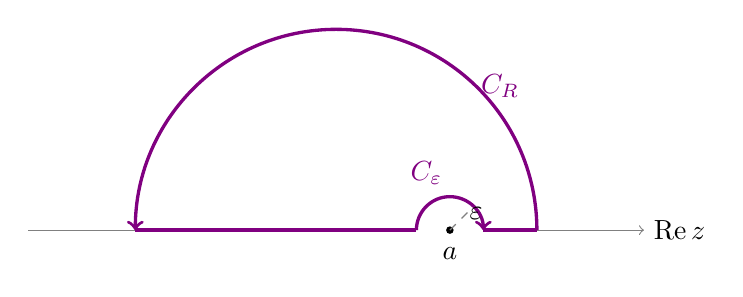
\begin{tikzpicture}[scale=0.85]
\draw[->,gray] (-4.6,0) -- (4.6,0) node[right,black]{$\mathrm{Re}\,z$};
\draw[white,line width=3pt] (1.15,0) -- (2.25,0);
\draw[violet,very thick] (-3,0) -- (1.2,0);
\draw[violet,very thick] (2.2,0) -- (3,0);
\draw[violet,very thick,->] (1.2,0) arc (180:0:0.5);
\draw[violet,very thick,->] (3,0) arc (0:180:3);
\node[violet] at (1.35,0.85) {$C_\varepsilon$};
\fill (1.7,0) circle (1.6pt);
\node[below] at (1.7,-0.12) {$a$};
\draw[dashed,gray] (1.7,0) -- (2.05,0.35);
\node[right] at (1.85,0.25) {$\varepsilon$};
\node[violet] at (2.45,2.15) {$C_R$};
\end{tikzpicture}
\end{center}

图上实轴在 $a$ 处被挖掉一段 $[a-\varepsilon,a+\varepsilon]$，用上半小半圆接起来；整条曲线仍然闭合，方向是“逆时针绕行、区域在左手边”。

\subhdr{3.2\quad 陈述}

\textbf{引理（小圆弧引理）}：设 $a$ 是实轴上的点，$f$ 在 $0<|z-a|<\rho$ 内解析，且 $a$ 是 $f$ 的\textbf{一阶}极点，记

$$
c=\operatorname{Res}f(a).
$$

设 $C_\varepsilon$ 是以 $a$ 为心、半径 $\varepsilon$ 的\textbf{上半}小半圆，按 $\theta$ 从 $\pi$ 减到 $0$ 的方向走（即从 $a-\varepsilon$ 沿上半平面走到 $a+\varepsilon$）。则

$$
\lim_{\varepsilon\to0}\int_{C_\varepsilon}f(z)\,\mathrm{d}z=-i\pi c .
$$

\subhdr{3.3\quad 证明}

把 $f$ 在 $a$ 附近写成“极点项 + 解析项”。一阶极点的洛朗展开是

$$
f(z)=\frac{c}{z-a}+g(z),
$$

其中 $g$ 在 $a$ 的邻域内解析（因而有界，记 $\max|g|=G$）。于是

$$
\int_{C_\varepsilon}f\,\mathrm{d}z
=c\int_{C_\varepsilon}\frac{\mathrm{d}z}{z-a}+\int_{C_\varepsilon}g\,\mathrm{d}z .
$$

\textbf{第一项}：令 $z=a+\varepsilon e^{i\theta}$，$\theta$ 从 $\pi$ 到 $0$，

$$
\int_{C_\varepsilon}\frac{\mathrm{d}z}{z-a}
=\int_{\pi}^{0}\frac{i\varepsilon e^{i\theta}}{\varepsilon e^{i\theta}}\,\mathrm{d}\theta
=i(0-\pi)=-i\pi .
$$

\textbf{第二项}：弧长 $\pi\varepsilon$，$|g|\le G$，由 ML 不等式

$$
\left|\int_{C_\varepsilon}g\,\mathrm{d}z\right|\le G\cdot\pi\varepsilon\to0 .
$$

两项相加，极限为 $-i\pi c$。

\aside{证明里只有一个“技术点”：$g$ 必须有界。一阶极点保证 $f-c/(z-a)$ 在 $a$ 处可去；若阶数更高，$g$ 里会留着 $1/(z-a)^2$ 这类项，它就不再是有界的了（见 3.6）。}

\subhdr{3.4\quad 一般张角}

若小弧从角 $\theta_1$ 转到 $\theta_2$（标准极角，逆时针为正），同样算法给出

$$
\int_{\text{小弧}}\frac{\mathrm{d}z}{z-a}=i(\theta_2-\theta_1).
$$

半圆对应 $\theta_2-\theta_1=\pm\pi$。所以小圆弧引理的本质是：\textbf{极点项 $\dfrac{c}{z-a}$ 在圆心角上的积分只与转过的角度有关}，半圆给 $\pm i\pi$，整圆给 $\pm2\pi i$（整圆的情形正是留数定理）。

\subhdr{3.5\quad 方向表}

四个方向分别算一次。极角都从正实轴起算、逆时针为正。

\begin{minipage}{\linewidth}
\small
\tabtop
\begin{tabular}{@{}llll@{}}
\thead{半圆位置} & \thead{走向} & \thead{$\theta$ 的变化} & \thead{积分值} \\
\end{tabular}
\tabmid
\begin{tabular}{@{}llll@{}}
上半 & 左 $\to$ 右 & $\pi\to0$ & $-i\pi c$ \\
上半 & 右 $\to$ 左 & $0\to\pi$ & $+i\pi c$ \\
下半 & 左 $\to$ 右 & $\pi\to2\pi$ & $+i\pi c$ \\
下半 & 右 $\to$ 左 & $2\pi\to\pi$ & $-i\pi c$ \\
\end{tabular}
\tabbot
\end{minipage}

\textbf{逐行读法}：每行都是 $i(\theta_{\text{终}}-\theta_{\text{始}})c$。第一行 $\theta$ 减小 $\pi$，给 $-i\pi c$；第二行增加 $\pi$，给 $+i\pi c$；第三行走下半圈、$\theta$ 从 $\pi$ 增大到 $2\pi$，给 $+i\pi c$；第四行从 $2\pi$ 回到 $\pi$，给 $-i\pi c$。

\textbf{边界行}：$\theta$ 变化恰好为 0（没绕过去）时积分为 0，这是“极点其实在围道外侧”的情形。

\textbf{一句话规则}：\textbf{$\theta$ 增大给 $+i\pi c$，$\theta$ 减小给 $-i\pi c$}，与半圆在上半还是下半无关。

\subhdr{3.6\quad 为什么必须是一阶}

如果 $a$ 是二阶极点，$f=\dfrac{c}{(z-a)^{2}}+\cdots$，第一项变成

$$
\int_{C_\varepsilon}\frac{\mathrm{d}z}{(z-a)^{2}}
=\int_{\pi}^{0}\frac{i\varepsilon e^{i\theta}}{\varepsilon^{2}e^{2i\theta}}\,\mathrm{d}\theta
=\frac{i}{\varepsilon}\int_{\pi}^{0}e^{-i\theta}\,\mathrm{d}\theta
=-\frac{2}{\varepsilon}\to-\infty .
$$

不再有有限极限。所以二阶及以上的极点落在围道上时，“半留数”这套办法失效，主值也可能不存在（除非题目按对称方式另行定义）。

\hdr{§3 续}{两个新概念：主值与半留数}

\subhdr{3.7\quad 柯西主值}

\textbf{为什么需要它}：$\displaystyle\int_{-\infty}^{\infty}\frac{\mathrm{d}x}{x}$ 作为普通广义积分是发散的（两端的对数各自发散）。但如果我们\textbf{对称地}挖掉原点，

$$
\lim_{\varepsilon\to0}\left(\int_{-\infty}^{-\varepsilon}+\int_{\varepsilon}^{\infty}\right)\frac{\mathrm{d}x}{x},
$$

两边的发散正好抵消，极限存在且等于 0。

\textbf{定义（柯西主值）}：设 $a$ 是 $f$ 在实轴上唯一的极点，若极限

$$
\mathrm{PV}\!\int_{-\infty}^{\infty}f(x)\,\mathrm{d}x
:=\lim_{\varepsilon\to0}\left(\int_{-\infty}^{a-\varepsilon}f+\int_{a+\varepsilon}^{\infty}f\right)
$$

存在，就称它为主值。多个实轴极点时，每个极点各用一个小 $\varepsilon$ 对称挖掉，再让所有 $\varepsilon\to0$。

\textbf{注意两件事}：主值是“一种约定的广义值”，不是普通积分；存在主值不代表积分收敛（上面的 $1/x$ 就是例子）。

\subhdr{3.8\quad 半留数与主值公式}

现在把围道拼起来：实轴（挖掉实轴极点）$+$ 各小半圆 $C_{\varepsilon,k}$ $+$ 上半大圆弧 $C_R$。设围道内部（上半平面）的奇点是 $z_j$，实轴上的极点是 $a_k$，则

$$
\oint_\Gamma f\,\mathrm{d}z
=2\pi i\sum_j\operatorname{Res}f(z_j).
$$

左边拆成三部分：

$$
\oint_\Gamma=\underbrace{\mathrm{PV}\!\int_{-\infty}^{\infty}f\,\mathrm{d}x}_{\text{实轴}}
+\underbrace{\sum_k\int_{C_{\varepsilon,k}}f}_{\to -i\pi\sum_k\operatorname{Res}f(a_k)}
+\underbrace{\int_{C_R}f}_{\to0}.
$$

（$C_R$ 那一项按 §2 或 §2.6 扔掉。）移项得

$$
\mathrm{PV}\!\int_{-\infty}^{\infty}f(x)\,\mathrm{d}x
=2\pi i\sum_{\text{上半平面}}\operatorname{Res}f
+i\pi\sum_{\text{实轴}}\operatorname{Res}f .
$$

第二项就是\textbf{半留数}：小半圆只绕过一圈的一半（角度 $\pi$，不是 $2\pi$），所以是 $i\pi$ 而不是 $2\pi i$。

\aside{符号核对：上半小半圆按“左 $\to$ 右”走（$\theta$ 减小），给 $-i\pi$，移到右边变成 $+i\pi$。如果题目要求从下方绕，符号相反，两个 $i\pi$ 项整体变号。}

\subhdr{3.9\quad 主值的三条性质}

\textbf{第一，主值是线性的}：$\mathrm{PV}(af+bg)=a\,\mathrm{PV}f+b\,\mathrm{PV}g$，只要右边两个主值都存在。

\textbf{第二，奇函数的主值为 0}：$\mathrm{PV}\!\int_{-\infty}^{\infty}\dfrac{\mathrm{d}x}{x}=0$。原因是挖洞是对称的，左右两段精确抵消。

\textbf{第三，主值存在不等于积分收敛}。$1/x$ 就是标准反例：普通积分发散，主值却是 0。写答案时若用了主值，必须标注 $\mathrm{PV}$，不能写成普通的 $\int$。

另外，\textbf{高阶极点的主值常常不存在}：例如

$$
\mathrm{PV}\!\int_{-\infty}^{\infty}\frac{\mathrm{d}x}{x^{2}}
=\lim_{\varepsilon\to0}\left(\int_{-\infty}^{-\varepsilon}+\int_{\varepsilon}^{\infty}\right)\frac{\mathrm{d}x}{x^{2}}
=\lim_{\varepsilon\to0}\frac{2}{\varepsilon}=+\infty ,
$$

对称挖洞也救不回来。这与 3.6 的结论一致：二阶极点在小弧上的积分本身就按 $1/\varepsilon$ 发散。

\hdr{§4}{例题}

\qbreak
\qstem{例 1（大圆弧，类型 2）计算 $\displaystyle I=\int_{-\infty}^{\infty}\frac{\mathrm{d}x}{1+x^{2}}$。}

\textbf{补弧}：上半大圆弧 $C_R$，围道 $\Gamma_R=[-R,R]+C_R$。上半平面只有一个一阶极点 $z=i$，$\operatorname{Res}f(i)=\dfrac{1}{2i}$。

\textbf{扔掉圆弧}：在 $C_R$ 上 $|1+z^{2}|\ge R^{2}-1$，所以

$$
M(R)=\frac{1}{R^{2}-1},\qquad R\,M(R)=\frac{R}{R^{2}-1}\to0 .
$$

大圆弧引理成立。于是

$$
I=2\pi i\cdot\frac{1}{2i}=\pi .
$$

\textbf{自检}：$\arctan x$ 在 $\pm\infty$ 的差是 $\pi$，一致。

\qbreak
\qstem{例 2（大圆弧引理失效）计算 $\displaystyle\int_{C_R}\frac{\mathrm{d}z}{z}$，$C_R$ 为上半大圆弧。}

参数化 $z=Re^{i\theta}$，$\theta$ 从 $0$ 到 $\pi$：

$$
\int_{C_R}\frac{\mathrm{d}z}{z}
=\int_0^{\pi}\frac{iRe^{i\theta}}{Re^{i\theta}}\,\mathrm{d}\theta
=i\pi .
$$

这里 $M(R)=1/R$，$R\,M(R)=1$ 不趋于 0，大圆弧引理不适用，而积分确实不消失。这个例子说明：\textbf{条件不满足时，结论可以真的不成立}，不能凭“$R$ 很大”想当然。

\qbreak
\qstem{例 3（两个引理合用）计算 $\displaystyle I=\int_0^{\infty}\frac{\sin x}{x}\,\mathrm{d}x$。}

\textbf{选函数}：$\sin x/x$ 在 $0$ 处可去，但围道要绕的是 $e^{iz}/z$ 的一阶极点 $0$。记 $f(z)=e^{iz}/z$。

\textbf{围道}：$[-R,-\varepsilon]+C_\varepsilon+[\varepsilon,R]+C_R$，其中 $C_\varepsilon$ 取上半小半圆、从 $-\varepsilon$ 走到 $+\varepsilon$（$\theta$ 从 $\pi$ 减到 $0$）。

\textbf{围道内部无奇点}（围道从上方绕开原点，原点在外部），所以

$$
\oint_\Gamma f\,\mathrm{d}z=0 .
$$

\textbf{三段极限}：

- $C_R$：$\left|1/z\right|\to0$ 一致，约当引理给 $\int_{C_R}\to0$；
- $C_\varepsilon$：一阶极点，小圆弧引理给 $\int_{C_\varepsilon}\to-i\pi\operatorname{Res}f(0)=-i\pi$；
- 实轴两段：合起来趋于主值 $\mathrm{PV}\!\int f$。

代入恒等式：

$$
\mathrm{PV}\!\int_{-\infty}^{\infty}\frac{e^{ix}}{x}\,\mathrm{d}x-i\pi=0
\ \Longrightarrow\
\mathrm{PV}\!\int_{-\infty}^{\infty}\frac{e^{ix}}{x}\,\mathrm{d}x=i\pi .
$$

\textbf{取虚部}：

$$
\mathrm{PV}\!\int_{-\infty}^{\infty}\frac{\sin x}{x}\,\mathrm{d}x=\pi .
$$

被积函数是偶函数，所以

$$
I=\frac{\pi}{2} .
$$

\qbreak
\qstem{例 4（方向练习）设 $a$ 是一阶极点，$C_\varepsilon$ 取在下半平面、从 $a-\varepsilon$ 经下方走到 $a+\varepsilon$，求 $\displaystyle\lim_{\varepsilon\to0}\int_{C_\varepsilon}\frac{c}{z-a}\,\mathrm{d}z$。}

下半、左 $\to$ 右：$\theta$ 从 $\pi$ 增大到 $2\pi$，由 3.4 的公式

$$
i(2\pi-\pi)c=+i\pi c .
$$

与上半“左 $\to$ 右”（$-i\pi c$）差一个符号。这也说明“顺时针、逆时针”的口诀容易记反，用 $\theta$ 的增减最稳。

\qbreak
\qstem{例 5（高阶极点为什么不行）计算 $\displaystyle\int_{C_\varepsilon}\frac{\mathrm{d}z}{z^{2}}$，$C_\varepsilon$ 为上半小半圆、$\theta$ 从 $\pi$ 到 $0$。}

$$
\int_{C_\varepsilon}\frac{\mathrm{d}z}{z^{2}}
=\int_{\pi}^{0}\frac{i\varepsilon e^{i\theta}}{\varepsilon^{2}e^{2i\theta}}\,\mathrm{d}\theta
=\frac{i}{\varepsilon}\int_{\pi}^{0}e^{-i\theta}\,\mathrm{d}\theta
=\frac{i}{\varepsilon}\cdot\frac{e^{-i\theta}}{-i}\Big|_{\pi}^{0}
=-\frac{2}{\varepsilon}\to-\infty .
$$

模按 $1/\varepsilon$ 发散，没有有限极限。所以二阶极点落在围道上时，不能套半留数。

\qbreak
\qstem{例 6（大圆弧 + 二阶留数）计算 $\displaystyle I=\int_{-\infty}^{\infty}\frac{\mathrm{d}x}{(1+x^{2})^{2}}$。}

\textbf{补弧}：同样的上半大圆弧。上半平面只有 $z=i$，是\textbf{二阶}极点。

\textbf{留数}（规则 III，$m=2$）：

$$
\operatorname{Res}f(i)=\lim_{z\to i}\frac{\mathrm{d}}{\mathrm{d}z}\left[\frac{1}{(z+i)^{2}}\right]
=\frac{-2}{(2i)^{3}}=\frac{1}{4i}.
$$

\textbf{扔掉圆弧}：$|1+z^{2}|\ge R^{2}-1$，所以 $|f|\le\dfrac{1}{(R^{2}-1)^{2}}$，

$$
R\,M(R)=\frac{R}{(R^{2}-1)^{2}}\to0 ,
$$

大圆弧引理成立。于是

$$
I=2\pi i\cdot\frac{1}{4i}=\frac{\pi}{2}.
$$

\textbf{自检}：令 $x=\tan\theta$ 也可以算，结果相同；被积函数是偶函数，$\int_0^\infty$ 就是 $\pi/4$。

\qbreak
\qstem{例 7（从下方绕的完整记账）用下半小半圆重新算 $\displaystyle\mathrm{PV}\!\int_{-\infty}^{\infty}\frac{e^{ix}}{x}\,\mathrm{d}x$，核对例 3 的结果。}

\textbf{围道}：$[-R,-\varepsilon]+C_\varepsilon^{\text{下}}+[\varepsilon,R]+C_R$，其中 $C_\varepsilon^{\text{下}}$ 从 $-\varepsilon$ 经下方走到 $+\varepsilon$（$\theta$ 从 $\pi$ 增大到 $2\pi$）。

\textbf{关键区别}：这次围道从下方绕过原点，\textbf{原点落在围道内部}，所以

$$
\oint_\Gamma\frac{e^{iz}}{z}\,\mathrm{d}z=2\pi i\operatorname{Res}f(0)=2\pi i .
$$

\textbf{三段极限}：

- $C_R$：约当引理，$\to0$；
- $C_\varepsilon^{\text{下}}$：$\theta$ 增大 $\pi$，给 $+i\pi$（§3.5 表第三行）；
- 实轴两段：$\to\mathrm{PV}$。

代入：

$$
\mathrm{PV}+i\pi=2\pi i
\ \Longrightarrow\
\mathrm{PV}\!\int_{-\infty}^{\infty}\frac{e^{ix}}{x}\,\mathrm{d}x=i\pi .
$$

与例 3 完全一致。\textbf{两件事都变了、结果不变}：上半绕时“内部无奇点、小弧给 $-i\pi$”，下半绕时“内部有奇点（$2\pi i$）、小弧给 $+i\pi$”，两次的等式都给出同一个 $i\pi$。

\aside{这条对照最值得记住：\textbf{“原点算不算内部”与“小弧给正还是给负”必须同时判断}。只改一个会得到相差 $2\pi i$ 的错误答案。}

\hdr{§5}{易错点}

\gapitem{一}{把 $M$ 取成弧上的最小值。$M$ 必须是\textbf{上界}；取错方向会把“不趋于 0”判成“趋于 0”。}

\gapitem{二}{弧长写成 $R$ 或 $2\pi R$。上半圆弧长是 $\pi R$；整圆才是 $2\pi R$。}

\gapitem{三}{以为“$R$ 很大”就自动为 0。$1/z$ 的大圆弧积分恒为 $i\pi$，与 $R$ 无关。}

\gapitem{四}{小圆弧的方向记反。用 $\theta$ 的增减：增大 $+i\pi c$，减小 $-i\pi c$。}

\gapitem{五}{把二阶极点也按半留数处理。$1/(z-a)^2$ 的小弧积分按 $1/\varepsilon$ 发散。}

\gapitem{六}{忘了主值是“约定值”。写答案时要注明 $\mathrm{PV}$；普通积分本身可能发散。}

\hdr{§6}{自检题（答案在附录 A）}

\begin{enumerate}
\item 在 $C_R$ 上 $|f(z)|\le M/R^{2}$，大圆弧积分是否一定趋于 0？给出 $R\,M(R)$ 的量级。
\item 判断：$f(z)=1/(z^{2}+1)$ 在 $C_R$ 上满足大圆弧引理的条件吗？为什么？
\item $C_\varepsilon$ 取上半、从 $a+\varepsilon$ 走到 $a-\varepsilon$（$\theta$ 从 $0$ 到 $\pi$），一阶极点 $a$ 的贡献是多少？
\item 若实轴上有两个一阶极点，主值公式里“半留数”那一项要乘几个 $i\pi$？
\item $\displaystyle\int_{C_R}\frac{z}{z^{2}+1}\mathrm{d}z$ 在 $R\to\infty$ 时趋于多少？用大圆弧引理判断是否合法。
\item 为什么 $\int_0^{\infty}\frac{\sin x}{x}\mathrm{d}x$ 不能直接用大圆弧引理，而必须先用约当引理？
\end{enumerate}

\hdr{§7}{一页速查}

- 大圆弧：$|f|\le M(R)$ 且 $R\,M(R)\to0$ $\Longrightarrow$ $\int_{C_R}f\to0$。判断只看“$|f|$ 是否比 $1/R$ 掉得快”。
- 约当：$|g|\to0$ 且带 $e^{imz}$（$m>0$）$\Longrightarrow$ $\int_{C_R}ge^{imz}\to0$。
- 小圆弧：一阶极点、角度变化 $\Delta\theta$ $\Longrightarrow$ $\int\to i\Delta\theta\cdot\operatorname{Res}$；半圆 $\Delta\theta=\pm\pi$。
- 主值公式：$\mathrm{PV}\!\int=2\pi i\sum_{\text{上半}}\operatorname{Res}+i\pi\sum_{\text{实轴}}\operatorname{Res}$。
- 记符号的口诀：$\theta$ 增大 $+i\pi$，$\theta$ 减小 $-i\pi$。

\flowerrule

\hdr{附录 A}{自检题答案}

\begin{enumerate}
\item 是。$M(R)=M/R^{2}$，$R\,M(R)=M/R\to0$，满足条件。
\item 满足。$|1+z^{2}|\ge R^{2}-1$，故 $|f|\le1/(R^{2}-1)$，$R\,M(R)=R/(R^{2}-1)\to0$。
\item $\theta$ 从 $0$ 增大到 $\pi$，由 3.4 得 $+i\pi\operatorname{Res}f(a)$。
\item 每个实轴一阶极点各贡献一项 $i\pi\operatorname{Res}$，所以是求和 $\sum_k i\pi\operatorname{Res}f(a_k)$，不是乘“个数”的 $i\pi$ 再乘一个总留数。
\item 不趋于 0，极限是 $i\pi$。理由是 $|f|\sim1/R$，$R\,M\sim1$，条件不满足；直接算更清楚：把 $f$ 拆成 $\dfrac{z}{z^{2}+1}=\dfrac12\left(\dfrac{1}{z-i}+\dfrac{1}{z+i}\right)$，两项各自的大弧积分都趋于 $i\pi$，所以整体趋于 $i\pi$。用闭合围道核对：实轴上 $\mathrm{PV}\!\int\dfrac{x}{x^{2}+1}\mathrm{d}x=0$（奇函数），闭合围道 $=i\pi=2\pi i\cdot\operatorname{Res}f(i)=2\pi i\cdot\dfrac12$，两边一致。
\item 因为 $|e^{iz}/z|=e^{-R\sin\theta}/R$ 在 $\theta\approx0,\pi$ 处约为 $1/R$，$R\,M$ 不趋于 0，大圆弧引理给不出零；约当引理利用 $\sin\theta$ 离开实轴后的指数衰减，才把它压到 0。
\end{enumerate}

\flowerrule

\hdr{附录 B}{四道补充练习（详解在题后）}

\textbf{B1.} 计算 $\displaystyle\int_{C_R}\frac{\mathrm{d}z}{z-a}$，其中 $a$ 是上半平面的固定点，$R>|a|$ 且 $R\to\infty$。

\textbf{解}：把被积函数在无穷远展开：

$$
\frac{1}{z-a}=\frac1z\cdot\frac{1}{1-a/z}=\frac1z+\frac{a}{z^{2}}+\frac{a^{2}}{z^{3}}+\cdots\qquad(|z|>|a|).
$$

第一项在弧上积分是 $i\pi$（例 2），后面各项满足大圆弧引理（$|a^{k}/z^{k+1}|\le |a|^{k}/R^{k+1}$，乘以 $\pi R$ 得 $\pi|a|^{k}/R^{k}\to0$）。所以

$$
\int_{C_R}\frac{\mathrm{d}z}{z-a}\to i\pi .
$$

\textbf{点评}：这个结果说明“大圆弧上的积分不一定为 0”，$1/z$ 型的主项总留下一个 $i\pi$。它也是留数定理在无穷远处那一条的几何来源。

\textbf{B2.} 用大圆弧引理计算 $\displaystyle I=\int_{-\infty}^{\infty}\frac{\mathrm{d}x}{x^{2}+2x+2}$。

\textbf{解}：配方 $x^{2}+2x+2=(x+1)^{2}+1$，上半平面的极点是 $z=-1+i$（一阶），

$$
\operatorname{Res}f(-1+i)=\frac{1}{2z+2}\Big|_{z=-1+i}=\frac{1}{2i}.
$$

在 $C_R$ 上，$|z^{2}+2z+2|\ge R^{2}-2R-2$（对充分大的 $R$），所以

$$
R\,M(R)\le\frac{R}{R^{2}-2R-2}\to0 ,
$$

大圆弧引理成立。于是

$$
I=2\pi i\cdot\frac{1}{2i}=\pi .
$$

\textbf{点评}：配方后就是 $\int\mathrm{d}u/(u^{2}+1)=\pi$，与平移无关——但用围道做一遍，是为了练“先找上半平面的极点”。

\textbf{B3.} 计算 $\displaystyle\mathrm{PV}\!\int_{-\infty}^{\infty}\frac{\mathrm{d}x}{x-1}$。

\textbf{解}：按定义，先挖掉 $x=1$，再对称截断到 $[-L,L]$：

$$
\int_{-L}^{1-\varepsilon}\frac{\mathrm{d}x}{x-1}+\int_{1+\varepsilon}^{L}\frac{\mathrm{d}x}{x-1}
=\ln\varepsilon-\ln(L+1)+\ln(L-1)-\ln\varepsilon
=\ln\frac{L-1}{L+1}.
$$

$\ln\varepsilon$ 两项\textbf{精确抵消}（因为挖洞是对称的），剩下的只依赖 $L$：

$$
\lim_{L\to\infty}\ln\frac{L-1}{L+1}=0 .
$$

所以主值存在，且

$$
\mathrm{PV}\!\int_{-\infty}^{\infty}\frac{\mathrm{d}x}{x-1}=0 .
$$

\textbf{点评}：每一段单独看都是对数发散的（左段 $\to-\infty$，右段 $\to+\infty$），但两个发散在对称挖洞下刚好抵消。这与 $\mathrm{PV}\int\mathrm{d}x/x=0$ 是同一件事（平移不变）。对比 §3.9 的 $1/x^{2}$：那里抵消不掉，主值发散——差别在于 $1/(x-a)$ 在极点两侧异号，而 $1/(x-a)^{2}$ 同号。

\textbf{B4.} 计算 $\displaystyle\int_{C_\varepsilon}\frac{\mathrm{d}z}{z-a}$，$C_\varepsilon$ 为下半小半圆、从 $a+\varepsilon$ 经下方走到 $a-\varepsilon$。

\textbf{解}：$\theta$ 从 $0$ 减到 $-\pi$（即从 $2\pi$ 减到 $\pi$），$\Delta\theta=-\pi$，所以

$$
\int=i(-\pi)=-i\pi .
$$

\textbf{点评}：与 §3.5 表的第四行一致（下半、右 $\to$ 左）。

\end{document}